\documentclass{article}
\usepackage{listings}
\usepackage{graphicx}
\usepackage{color}

\definecolor{mygreen}{rgb}{0,0.6,0}
\definecolor{mygray}{rgb}{0.5,0.5,0.5}
\definecolor{mymauve}{rgb}{0.58,0,0.82}

\lstset{ %
  backgroundcolor=\color{white},   % choose the background color; you must add \usepackage{color} or \usepackage{xcolor}; should come as last argument
  basicstyle=\footnotesize,        % the size of the fonts that are used for the code
  breakatwhitespace=false,         % sets if automatic breaks should only happen at whitespace
  breaklines=true,                 % sets automatic line breaking
  captionpos=b,                    % sets the caption-position to bottom
  commentstyle=\color{mygreen},    % comment style
  deletekeywords={...},            % if you want to delete keywords from the given language
  escapeinside={\%*}{*)},          % if you want to add LaTeX within your code
  extendedchars=true,              % lets you use non-ASCII characters; for 8-bits encodings only, does not work with UTF-8
  frame=single,	                   % adds a frame around the code
  keepspaces=true,                 % keeps spaces in text, useful for keeping indentation of code (possibly needs columns=flexible)
  keywordstyle=\color{blue},       % keyword style
  language=Octave,                 % the language of the code
  morekeywords={*,...},           % if you want to add more keywords to the set
  numbers=left,                    % where to put the line-numbers; possible values are (none, left, right)
  numbersep=5pt,                   % how far the line-numbers are from the code
  numberstyle=\tiny\color{mygray}, % the style that is used for the line-numbers
  rulecolor=\color{black},         % if not set, the frame-color may be changed on line-breaks within not-black text (e.g. comments (green here))
  showspaces=false,                % show spaces everywhere adding particular underscores; it overrides 'showstringspaces'
  showstringspaces=false,          % underline spaces within strings only
  showtabs=false,                  % show tabs within strings adding particular underscores
  stepnumber=2,                    % the step between two line-numbers. If it's 1, each line will be numbered
  stringstyle=\color{mymauve},     % string literal style
  tabsize=2,	                   % sets default tabsize to 2 spaces
  title=\lstname                   % show the filename of files included with \lstinputlisting; also try caption instead of title
}

\author{Jacob Hutter}
\title{ECE 311 Lab 3}

\begin{document}
\maketitle

\begin{figure}[H]
\lstinputlisting[language=Matlab]{myDFTConv.m}
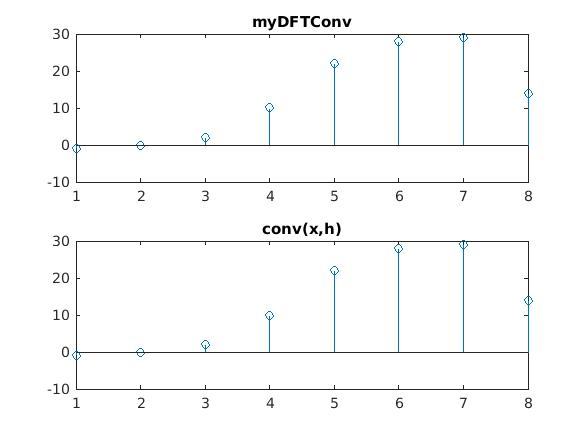
\includegraphics[scale = .5]{report1}
\\ Because of the use of fft and ifft, the time coplexity is also $O(Nlog(N))$.
\end{figure}



\begin{figure}[H]
\lstinputlisting[language=Matlab]{sys1.m}
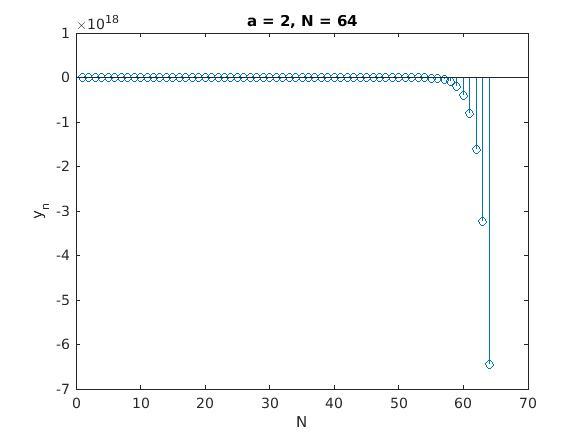
\includegraphics[scale = .5]{report2}
\\ Notice that this function is in the order of $-e^x$ 
therefore, it is not stable $\lim_{x_n\to\infty} y_n = -\infty$.
The system is causal, however, by the finite difference equation, output only 
depends on past or current inputs.
\end{figure}

\begin{figure}[H]
\lstinputlisting[language=Matlab]{sys2.m}
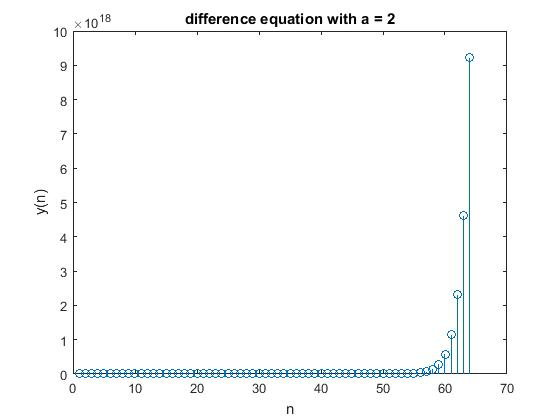
\includegraphics[scale = .5]{report3}

\end{figure}

\begin{figure}[H]
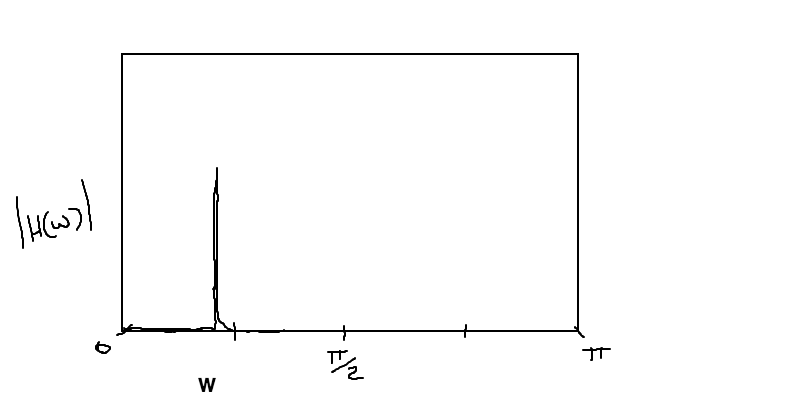
\includegraphics[scale = .5]{report4_1}
\ We can see on the interval from $w = 0$ to $pi$, that there is only one point where the magnitude is not zero. Therefore, there is a spike at that point.
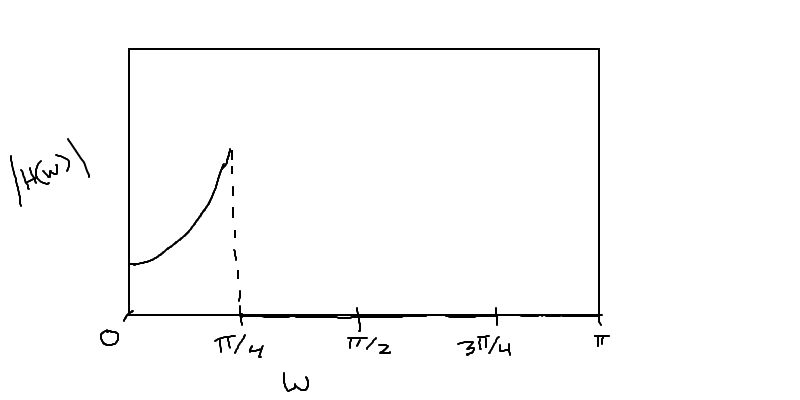
\includegraphics[scale = .5]{report4_2}
\ We can see on the interval from $w = 0$ to $Pi$ that there is a minimum at $omega = 0$ and a maximum at ~$w = pi/4$ so the graph is increasing until that point.
\end{figure}

\begin{figure}[H]
\lstinputlisting[language=Matlab]{pzplot_impz.m}
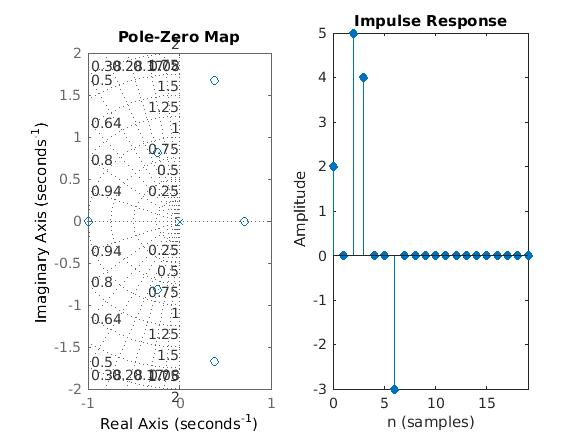
\includegraphics[scale = .5]{report5_1}
\ With $a = [1,0,0,0,0,0,0]$ and $b =[2,0,5,4,0,0,-3]$
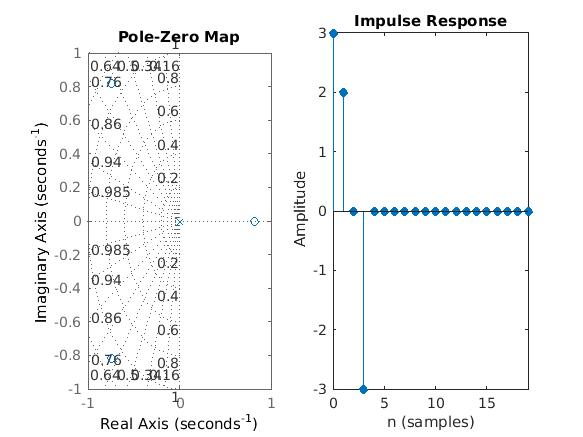
\includegraphics[scale = .5]{report5_2}
\ With $a = [1,0,0,0]$ and $b = [3,2,0,-3]$
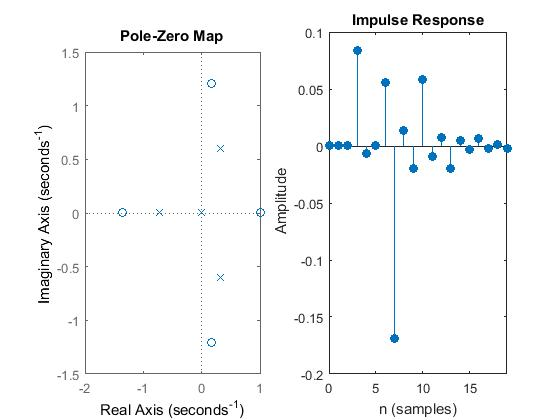
\includegraphics[scale = .5]{report5_3}
\ With $a = [12,1,0,4,0,0,0,0]$ and $b =[0,0,0,1,0,0,1,-2]$
\
\end{figure}



\break

\end{document}
